\begin{figure}
	\scalebox{1.5}{
		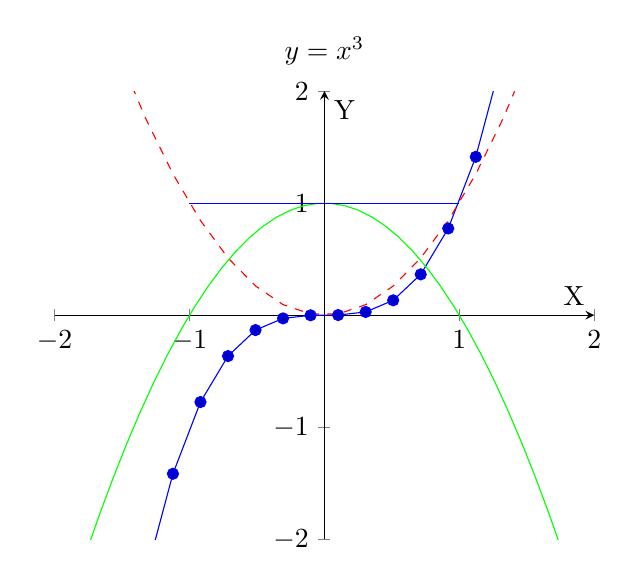
\begin{tikzpicture}
			\begin{axis}[
					xmin=-2, xmax=2, ymin=-2, ymax=2,
					axis lines=middle,
					samples=50,
					title={$y=x^3$},
					xlabel={X},
					ylabel={Y}
				]
				\addplot{x^3};
				\addplot[color=red, dashed]{x^2};
				\addplot[color=green, samples=100]{1-x^2};
				\addplot[color=blue, domain=-1:1]{1};
			\end{axis}
		\end{tikzpicture}
	}
	\caption{Примеры графиков разными линиями}
\end{figure}
